\documentclass[final,dvipsnames]{beamer}
\usepackage{amsmath,amsfonts,amssymb,pxfonts,eulervm,xspace}
\usepackage{graphicx,subfigure,comment,tikz}
\usepackage{array}
\usepackage{adjustbox}
\usepackage{framed}
\usepackage{xcolor}
\usepackage{mdframed}
\usepackage{multirow}
\usepackage{svaiter}
\usepackage[utf8]{inputenc}
\usepackage{arydshln}
\usepackage{relsize}
\usepackage{ragged2e}

\graphicspath{{./img/}}
\usepackage[orientation=landscape,size=a0,scale=1.5,debug]{beamerposter}

\mode<presentation>{\usetheme{inriaposter}}

\makeatletter
\pgfkeys{/pgf/.cd,
  parallelepiped offset x/.initial=2mm,
  parallelepiped offset y/.initial=2mm
}
\pgfdeclareshape{parallelepiped}
{
  \inheritsavedanchors[from=rectangle] % this is nearly a rectangle
  \inheritanchorborder[from=rectangle]
  \inheritanchor[from=rectangle]{north}
  \inheritanchor[from=rectangle]{north west}
  \inheritanchor[from=rectangle]{north east}
  \inheritanchor[from=rectangle]{center}
  \inheritanchor[from=rectangle]{west}
  \inheritanchor[from=rectangle]{east}
  \inheritanchor[from=rectangle]{mid}
  \inheritanchor[from=rectangle]{mid west}
  \inheritanchor[from=rectangle]{mid east}
  \inheritanchor[from=rectangle]{base}
  \inheritanchor[from=rectangle]{base west}
  \inheritanchor[from=rectangle]{base east}
  \inheritanchor[from=rectangle]{south}
  \inheritanchor[from=rectangle]{south west}
  \inheritanchor[from=rectangle]{south east}
  \backgroundpath{
    % store lower right in xa/ya and upper right in xb/yb
    \southwest \pgf@xa=\pgf@x \pgf@ya=\pgf@y
    \northeast \pgf@xb=\pgf@x \pgf@yb=\pgf@y
    \pgfmathsetlength\pgfutil@tempdima{\pgfkeysvalueof{/pgf/parallelepiped offset x}}
    \pgfmathsetlength\pgfutil@tempdimb{\pgfkeysvalueof{/pgf/parallelepiped offset y}}
    \def\ppd@offset{\pgfpoint{\pgfutil@tempdima}{\pgfutil@tempdimb}}
    \pgfpathmoveto{\pgfqpoint{\pgf@xa}{\pgf@ya}}
    \pgfpathlineto{\pgfqpoint{\pgf@xb}{\pgf@ya}}
    \pgfpathlineto{\pgfqpoint{\pgf@xb}{\pgf@yb}}
    \pgfpathlineto{\pgfqpoint{\pgf@xa}{\pgf@yb}}
    \pgfpathclose
    \pgfpathmoveto{\pgfqpoint{\pgf@xb}{\pgf@ya}}
    \pgfpathlineto{\pgfpointadd{\pgfpoint{\pgf@xb}{\pgf@ya}}{\ppd@offset}}
    \pgfpathlineto{\pgfpointadd{\pgfpoint{\pgf@xb}{\pgf@yb}}{\ppd@offset}}
    \pgfpathlineto{\pgfpointadd{\pgfpoint{\pgf@xa}{\pgf@yb}}{\ppd@offset}}
    \pgfpathlineto{\pgfqpoint{\pgf@xa}{\pgf@yb}}
    \pgfpathmoveto{\pgfqpoint{\pgf@xb}{\pgf@yb}}
    \pgfpathlineto{\pgfpointadd{\pgfpoint{\pgf@xb}{\pgf@yb}}{\ppd@offset}}
  }
}
\makeatother

%-- Header and footer information ----------------------------------
\newcommand{\footleft}{\footnotesize nicolas.keriven@gipsa-lab.grenoble-inp.fr, alberto@bietti.me, samuel.vaiter@u-bourgogne.fr}
\newcommand{\footright}{\footnotesize This work was supported by ANR GraVa ANR-18-CE40-0005 and ANER RAGA G048CVCRB2018ZZ.}
\title{Convergence and Stability of Graph Convolutional Networks on Large Random Graphs}
\author{Nicolas Keriven$^1$, Alberto Bietti$^2$, Samuel Vaiter$^3$}
\institute{$^1$CNRS, GIPSA-lab, Grenoble\quad $^2$NYU Center for Data Science, New York\quad $^3$CNRS, IMB, Dijon
}
\newcommand{\vsp}{\vspace{10pt}}
\newcommand{\vspp}{\vspace{-10pt}}
\usetikzlibrary{arrows.meta}
%-------------------------------------------------------------------

\newcommand{\cita}[1]{{\footnotesize \emph{(#1)}}}

\newcommand{\myemph}[1]{\textcolor{red}{#1}}
\newcommand{\myemphh}[1]{\textbf{\textcolor{red}{#1}}}
\newcommand{\mycolbacksum}[1]{
\hspace*{.01\linewidth}\begin{minipage}{.96\linewidth}
\begin{mdframed}[backgroundcolor=blue!10,linewidth=0pt]
\vsp
#1
%\vsp
\end{mdframed}
\end{minipage}
}
\newcommand{\mycolback}[1]{
\hspace*{.01\linewidth}\begin{minipage}{.96\linewidth}
\begin{mdframed}[backgroundcolor=blue!10,linewidth=0pt]
\vsp
#1
\vsp
\end{mdframed}
\end{minipage}
}
\newcommand{\mycolbackk}[1]{
\hspace*{.01\linewidth}\begin{minipage}{.96\linewidth}
\begin{mdframed}[backgroundcolor=red!10,linewidth=0pt]
\vsp
#1
\vsp
\end{mdframed}
\end{minipage}
}
\newcommand{\mycolbackwhite}[1]{
\hspace*{.01\linewidth}\begin{minipage}{.96\linewidth}
\begin{mdframed}[backgroundcolor=white,linewidth=1pt]
\vsp
#1
\vsp
\end{mdframed}
\end{minipage}
}
\usetikzlibrary{decorations.pathreplacing}

\begin{document}
\begin{frame}{}
\vspace{-40pt}
\begin{columns}[t]
%%%%%%%%%%%%%%%%%%%%%%%%%%%%%%%%%%%%%%%%%%%%%%%%%%%%%%%%%%%%%%%%%%%%%%%%%%%%%%%%%
\begin{column}{0.25\linewidth}
\begin{myalertblock}{1: Summary}
\begin{center}
\mycolbacksum{We study the \myemphh{convergence} of \textbf{Graph Convolutional Networks (GCNs)} to their \myemphh{continuous counterpart} as the number of nodes grows for a \myemphh{random graph} model, and derive \myemphh{stability} properties for realistic perturbations of the model.}
\end{center}
\vsp 

\hspace*{.01\linewidth}\begin{minipage}{.96\linewidth}
\mycolbackwhite{
Classical ``isomorphism-based'' analyses of GCN [2] or discrete stability bounds [4] are not entirely satisfying on \textbf{large} graphs. \myemphh{How do GCNs interact with (statistical models of) large graphs?}
}
\end{minipage}
\vsp

\begin{itemize}
\item We characterize GCNs on \textbf{latent position random graphs} as the number of nodes grows;
\item Results are non-asymptotic and valid for \textbf{relatively sparse} graphs (logarithmic degrees);
\item Analyze the stability of GCNs to \textbf{small deformations} of the random graph model.
\end{itemize}

\end{myalertblock}
\vsp 

\begin{myalertblock}{3: Convergence to continuous GCNs}

%\begin{itemize}
%  \item Output of GCN on random graph $\approx$ output of continuous GCN.
%\end{itemize}

\vspace{0.3cm}
\mycolback{
\textbf{Theorem}
  Let $(A,Z) \sim \Gamma$ with~$n$ nodes be drawn from~$\Gamma$. When $\alpha_n \gtrsim \log n/n$, with probability $1-n^{-r}$ for some $r>0$, we have
  \vsp
  \begin{equation*}
\left. \begin{matrix*}[r]
\sqrt{\frac{1}{n} \sum_i (\Phi_A(Z)_i - \Phi_{W,P}(f)(x_i))^2} \\
\| \bar \Phi_A(Z) - \bar \Phi_{W,P}(f)\|_2
\end{matrix*}\right\rbrace  \leq R_n
  \end{equation*}
  \vsp
  where {\color{red}$R_n = O(d n^{-\frac12} + (n\alpha_n)^{-\frac12})$}.
}

\vspace{1cm}
Numerical illustration\\
%Numerical illustration (Random graph with 3D latent positions)\\
  \small
  Equivariant GCN output for constant input $f=1$ with growing number of nodes and convergence with different sparsity levels $\alpha_{n}$\\
  \begin{center}
  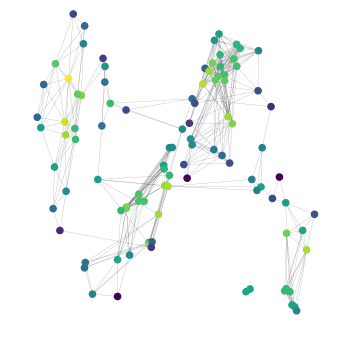
\includegraphics[width=0.28\linewidth]{img/cgcn_conv_illus0crop.png}\quad
  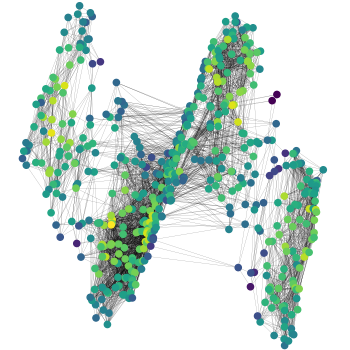
\includegraphics[width=0.28\linewidth]{img/cgcn_conv_illus1crop.png}\quad
  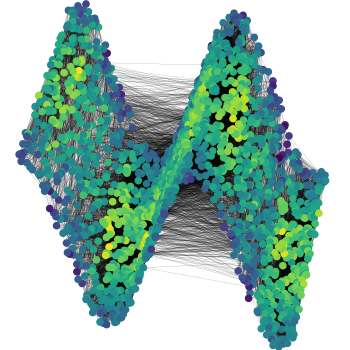
\includegraphics[width=0.28\linewidth]{img/cgcn_conv_illus2crop.png}\\ \vspace{1cm}
  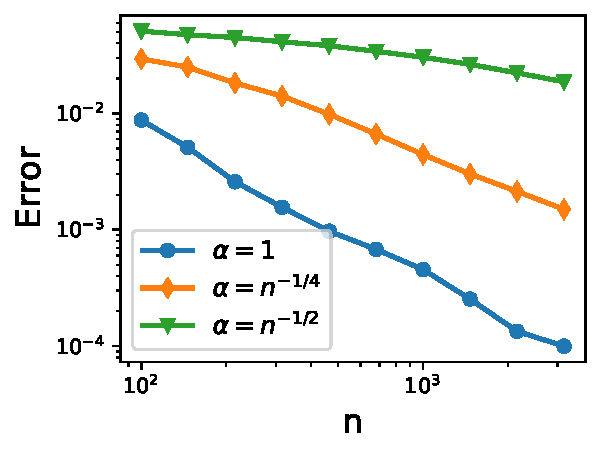
\includegraphics[width=0.48\linewidth]{img/illus_cv.pdf}
\end{center}
\end{myalertblock}

%\begin{mynotablock}{Notations}
%\begin{itemize}
%\item \textbf{Filter}: $h:\RR\to\RR,\quad h(\lambda) = \textstyle \sum_{k\geq 0} \beta_k \lambda^k$
%\item \textbf{Non-linearity}: $\rho: \RR \to \RR$, \emph{e.g.} ReLu
%\end{itemize}
%Graph theory
%\begin{itemize}
%\item \textbf{Graph}: $G = (A,Z)$, \textbf{Signals}: $Z \in \RR^{n \times d_z}$
%\item \textbf{Adjacency and degree}: $A \in \{0,1\}^{n \times n}$
%\end{itemize}
%\vsp
%Invariance
%\begin{itemize}
%\item \textbf{Permutation}: bijection $\sigma:[n] \to [n] \in \Sigma_n$
%\item \myemphh{Invariant function}: $f(\sigma \star W) = f(W)$
%\item \myemphh{Equivariant function}: $f(\sigma \star W) = \sigma\star f(W)$
%\end{itemize}
%\vsp
%Measure space
%\begin{itemize}
%  \item \textbf{Push-forward}: $f_{\sharp} \mu$
%  \item \textbf{Wasserstein-2 metric}: $\mathcal{W}_2$
%\end{itemize}
%\end{mynotablock}

%\begin{block}{Random graphs}
%\begin{itemize}
%  \item $(\Xx, d)$ compact metric space.
%  \item \textbf{random graph model:} $\Gamma=(P,W,f)$ 
%  \begin{itemize}
%    \item probability distribution $\Px$ over $\Xx$
%    \item symmetric kernel $W:\Xx\times \Xx \to [0,1]$
%    \item bounded function $f:\Xx\to \RR^{d_z}$.
%  \end{itemize}
%  
%  \item sparsity factor: $\alpha_n \in [0,1]$
%\end{itemize}
%\begin{equation*}
%  \forall j<i\leq n: \, x_i \stackrel{iid}{\sim} \Px, \,  z_{i} = f(x_i), \, a_{ij} \sim \Ber(\alpha_n W(x_i, x_j))
%\end{equation*}
%\end{block}

\end{column}%1




%%%%%%%%%%%%%%%%%%%%%%%%%%%%%%%%%%%%%%%%%%%%%%%%%%%%%%%%%%%%%%%%%%%%%%%%%%%%%%%%%%%%%%%%%%%%%%
\begin{column}{0.45\linewidth}

\begin{block}{2: \emph{Latent Positions} Random Graphs and Continuous GCN}

% \mycolbackwhite{
%\begin{table}
%\large
%\begin{tabular}{lcc}
% & \textbf{Discrete} & \textbf{Continuous} \\
% % \hline
%% \vspace{1cm} \\
%\textbf{Graph} \\
%Nodes & $i \in \{1, \ldots, n\}$ & $x \in \Xx$ \\
%Edges & $A_{ij}$ & $W(x, x')$ \\
%Degrees & $D_i = \sum_j A_{ij}$ & $d(x) = \int W(x, x')\mathrm{d} P(x')$ \\
%normalized Laplacian & $L= D^{-\frac12} A D^{-\frac12}$ & $\Ll f = \int \frac{W(\cdot, x)}{\sqrt{d(\cdot)d(x)}} f(x)\mathrm{d}P(x)$ \\
%\vspace{1cm} \\
%\textbf{GCN} \\
%Signal & $z_{i}^{\ell} \in \RR^{n}$ & $f_{i}^{\ell}: \mathcal{X} \to \RR$ \\
%Layer & {\normalsize $z_j^{(\ell+1)} = \rho\pa{\sum_i h^{(\ell)}_{ij}L z_i^{(\ell)}}$}
%    & $f_j^{(\ell+1)} = \rho\pa{\sum_i h^{(\ell)}_{ij}\Ll f_i^{(\ell)}}$ \\
%\vspace{1cm} \\
%\textbf{Representations} \\
%Equivariant GCN & \multicolumn{1}{l}{$\gcneq_A(Z) = Z^{(M)} \theta$} & \multicolumn{1}{l}{$\cgcneq_{W,P}(f) = \theta^\top f^{(M)}$} \\
%Invariant GCN & \multicolumn{1}{l}{$\gcninv_A(Z) = \frac{1}{n}\sum_{i=1}^n \gcneq_A(Z)_i$} & \multicolumn{1}{l}{$\cgcninv_{W,P}(f) = \int \cgcneq_{W,P}(f) \mathrm{d}P$}
%\end{tabular}
%\end{table}

\renewcommand{\arraystretch}{1.2}
\def\lsi{0.45}
\def\rsi{0.53}
\begin{table}
\large
\begin{tabular}{p{\lsi\textwidth}|p{\rsi\textwidth}}
\Centering{\myemphh{Graphs}} & \Centering{\myemphh{Random Graphs}} \\
\hline
\vspace{-2.5cm}
\begin{equation*}
G=(A,Z)
\end{equation*}

\parbox{\lsi\textwidth}{\normalsize
\vsp
\begin{itemize}
\item Adjacency matrix $A \in \{0,1\}^{n\times n}$
\item Signal over nodes $Z \in \mathbb{R}^{n\times d_0}$
\end{itemize}
}
&
\vspace{-2.5cm}
\begin{equation*}
\Gamma=(W,P,f)
\end{equation*}

\parbox{\rsi\textwidth}{\normalsize
\vsp
\begin{itemize}
\item Connectivity kernel $W: \mathcal{X} \times \Xx \to [0,1]$
\item Distribution $P$ over $\mathcal{X} \subset \mathbb{R}^d$
\item Function $f:\mathcal{X} \to \mathbb{R}^{d_0}$
\end{itemize}
\vspace{1cm}
}
\\
\hdashline
\parbox{\lsi\textwidth}{\normalsize
\vsp
\begin{itemize}
\item Degrees $D = \diag(A 1_n)$
\item Norm. Laplacian $L=D^{-\frac12} A D^{-\frac12}$
%\item Poly. filters $h(L) = \sum_{k\geq 0} \beta_k L^k$
\end{itemize}
}
&
\parbox{\rsi\textwidth}{\normalsize
\vsp
\begin{itemize}
\item Degree \textbf{function} $d = \int W(\cdot,x)\mathrm{d}P(x)$
\item Norm. Laplacian
$
\Ll f = \int \frac{W(\cdot, x)}{\sqrt{d(\cdot)d(x)}} f(x)\mathrm{d}P(x)
$
\end{itemize}
}\\
\hdashline
\end{tabular}

\parbox{\textwidth}{\vsp \vsp
\textbf{Generative model}
\begin{equation*}
{\color{red}  x_i \stackrel{iid}{\sim} \Px, \quad  z_{i} = f(x_i), \quad a_{ij} \sim \Ber(\alpha_n W(x_i, x_j))}
\end{equation*}
%
%%\parbox{\rsi\textwidth}{\normalsize
%%\vsp
\normalsize
\begin{itemize}
\item Dense $\alpha_n =O(1)$, Sparse $\alpha_n = O(1/n)$, \alert{Relatively sparse} $\alpha_n = O(\log n/n)$
\item Includes ER, SBM, $\varepsilon$-graphs, Gaussian kernel...
\end{itemize}
%%}
\begin{center}
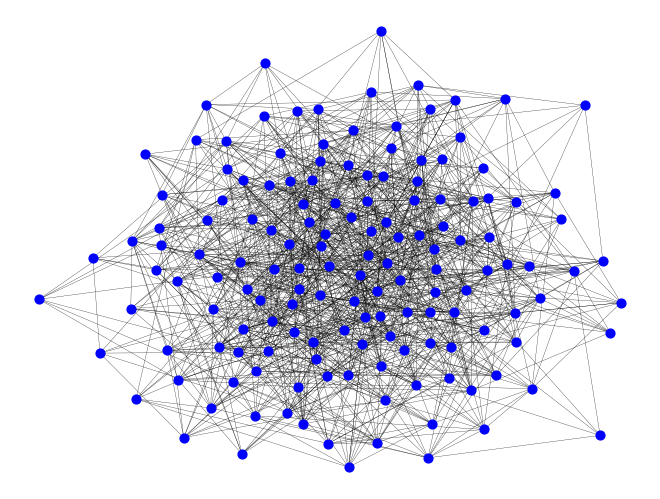
\includegraphics[height=8cm]{img/ex_ER.png}\quad
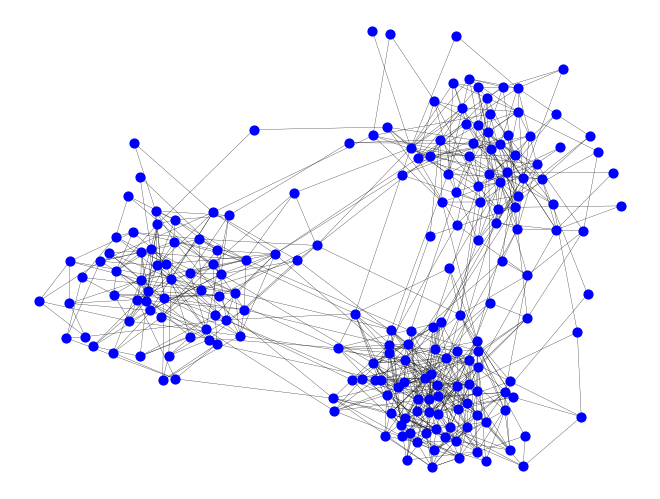
\includegraphics[height=8cm]{img/ex_SBM.png}\quad
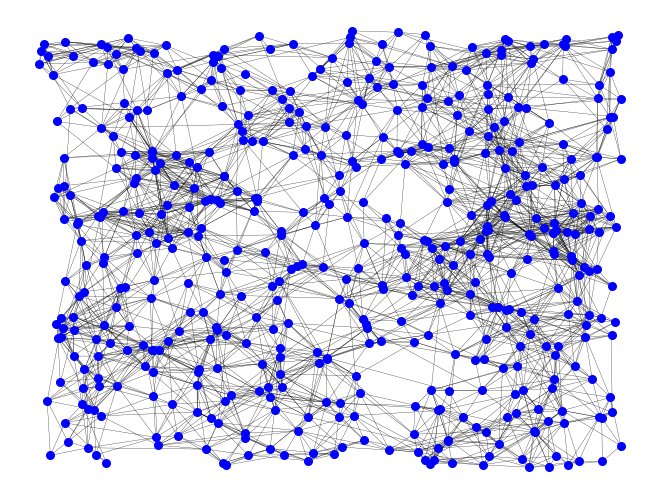
\includegraphics[height=8cm]{img/ex_Gauss.png}\quad
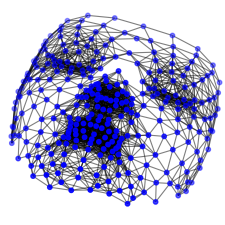
\includegraphics[height=8cm]{img/ex_eps.png}
\end{center}

}

\begin{tabular}{p{\lsi\textwidth}|p{\rsi\textwidth}}
\hdashline
\textbf{Isomorphism}
\begin{equation*}
(A, Z) ~\sim~ (\sigma A \sigma^\top, \sigma Z)
\end{equation*}

\parbox{\lsi\textwidth}{\normalsize
\vsp
\begin{itemize}
\item Permutation matrix $\sigma \in \{0,1\}^{n\times n}$
\end{itemize}
\vsp
}
&
\textbf{Continuous isomorphism}
\begin{equation*}
(P,W,f) ~\sim~ (\varphi^{-1}_\sharp P, W \circ \varphi^{\otimes 2}, f \circ \varphi)
\end{equation*}

\parbox{\rsi\textwidth}{\normalsize
\vsp
\begin{itemize}
\item Bijection $\varphi : \mathcal{X} \to \mathcal{X}$
\end{itemize}
\vsp
}
\\

\hline \hline
\Centering \myemphh{(Spectral) GCNs} & \Centering \myemphh{Continuous-GCNs (c-GCNs)} \\ \hline
\parbox{\rsi\textwidth}{\normalsize \vsp
\begin{itemize}
\item Propagate \textbf{signal over nodes}
\item Poly. filters $h(L) = \sum_k \beta_k L^k$
\end{itemize}
}
&
\parbox{\rsi\textwidth}{\normalsize \vsp
\begin{itemize}
\item Propagate \myemphh{function over latent space}
\item Poly. filters with $\mathcal{L}^k = \mathcal{L} \circ \ldots \circ \mathcal{L}$
\end{itemize}
}
\\
\vspace{-2.5cm}
\begin{equation*}
\mathsmaller{z_j^{(\ell+1)} = \rho\pa{\sum_i h^{(\ell)}_{ij}(L) z_i^{(\ell)} + b^{(\ell)}_j 1_n}}
\end{equation*}
\vspace{-1cm}
&
\vspace{-2.5cm}
\begin{equation*}
{\color{red}\mathsmaller{f_j^{(\ell+1)} = \rho\pa{\sum_i h^{(\ell)}_{ij}(\Ll) f_i^{(\ell)} + b^{(\ell)}_j}}}
\end{equation*}
\vspace{-1cm}
\\
\hdashline
\textbf{Equivariant output}
\begin{equation*}
\mathsmaller{\gcneq_A(Z) = Z^{(M)} \theta + 1_n b^\top}
\end{equation*}

\parbox{\lsi\textwidth}{\normalsize
\vsp
\begin{itemize}
\item $\gcneq_{\sigma A \sigma^\top}(\sigma Z) = \sigma \gcneq_A(Z)$
\end{itemize}
\vsp
}
&
\textbf{Equivariant output}
\begin{equation*}
\mathsmaller{\gcneq_{W,P}(f) = f^{(M)} \theta + b}
\end{equation*}

\parbox{\lsi\textwidth}{\normalsize
\vsp
\begin{itemize}
\item $\gcneq_{W \circ \varphi^{\otimes 2}, \varphi^{-1}_\sharp P}(f \circ \varphi) = \gcneq_{W,P}(f) \circ \varphi$
\end{itemize}
\vsp
}
\\
\hdashline
\textbf{Invariant output}
\begin{equation*}
\mathsmaller{\gcninv_A(Z) = 1_n^\top \gcneq_A(Z)}
\end{equation*}

\parbox{\lsi\textwidth}{\normalsize
\vsp
\begin{itemize}
\item $\gcninv_{\sigma A \sigma^\top}(\sigma Z) = \gcninv_A(Z)$
\end{itemize}
}
&
\textbf{Invariant output}
\begin{equation*}
\mathsmaller{\gcninv_{W,P}(f) = \int \cgcneq_{W,P}(f) \mathrm{d}P}
\end{equation*}

\parbox{\lsi\textwidth}{\normalsize
\vsp
\begin{itemize}
\item $\gcninv_{W \circ \varphi^{\otimes 2}, \varphi^{-1}_\sharp P}(f \circ \varphi) = \cgcninv_{W,P}(f)$
\end{itemize}
}
\\

%Degrees & $D_i = \sum_j A_{ij}$ & $d(x) = \int W(x, x')\mathrm{d} P(x')$ \\
%normalized Laplacian & $L= D^{-\frac12} A D^{-\frac12}$ & $\Ll f = \int \frac{W(\cdot, x)}{\sqrt{d(\cdot)d(x)}} f(x)\mathrm{d}P(x)$ \\
%\vspace{1cm} \\
%\textbf{GCN} \\
%Signal & $z_{i}^{\ell} \in \RR^{n}$ & $f_{i}^{\ell}: \mathcal{X} \to \RR$ \\
%Layer & {\normalsize $z_j^{(\ell+1)} = \rho\pa{\sum_i h^{(\ell)}_{ij}L z_i^{(\ell)}}$}
%    & $f_j^{(\ell+1)} = \rho\pa{\sum_i h^{(\ell)}_{ij}\Ll f_i^{(\ell)}}$ \\
%\vspace{1cm} \\
%\textbf{Representations} \\
%Equivariant GCN & \multicolumn{1}{l}{$\gcneq_A(Z) = Z^{(M)} \theta$} & \multicolumn{1}{l}{$\cgcneq_{W,P}(f) = \theta^\top f^{(M)}$} \\
%Invariant GCN & \multicolumn{1}{l}{$\gcninv_A(Z) = \frac{1}{n}\sum_{i=1}^n \gcneq_A(Z)_i$} & \multicolumn{1}{l}{$\cgcninv_{W,P}(f) = \int \cgcneq_{W,P}(f) \mathrm{d}P$}
\end{tabular}
\end{table}
% }

% \mycolbackwhite{
% Degree matrix $D = \diag(A 1_n)$\\
% normalized Laplacian matrix $L= D^{-\frac12} A D^{-\frac12}$
% \begin{equation*}
%   \forall j = 1,\ldots d_{\ell+1}, \quad z^{(\ell+1)}_j = \rho\pa{\sum_{i=1}^{d_\ell} h^{(\ell)}_{ij}(L) z^{(\ell)}_i + b_{j}^{(\ell)} 1_n } \in \RR^{n}
% \end{equation*}
% \begin{align*}
%   &\text{Equivariant GCN} && \text{Invariant GCN} \\
%   &\gcneq_A(Z) \eqdef Z^{(M)} \theta + 1_n b^\top && \gcninv_A(Z) \eqdef \frac{1}{n}\sum_{i=1}^n \gcneq_A(Z)_i
% \end{align*}
% }


% \mycolbackwhite{
% Degree function $d_{W} = \int W(\cdot, x)\mathrm{d} P(x)$\\
% normalized Laplacian operator $\Ll_{W,P} f = \int W(\cdot, x) f(x)/\sqrt{d_{W}(\cdot)d_{W}(x)}\mathrm{d}P(x)$.
% \begin{equation*}
%   \forall j=1,\ldots, d_{\ell+1}, \quad f^{(\ell+1)}_j = \rho \circ \pa{\sum_{i=1}^{d_\ell} h^{(\ell)}_{ij}(\Ll_{W,P}) f^{(\ell)}_i + b_{j}^{(\ell)}1(\cdot) }
% \end{equation*}
% \begin{align*}
%   &\text{Equivariant GCN} && \text{Invariant GCN} \\
%   & \cgcneq_{W,P}(f) \eqdef \theta^\top f^{(M)} + b 1(\cdot) && \cgcninv_{W,P}(f) = \int \cgcneq_{W,P}(f)(x)\mathrm{d}P(x)
% \end{align*}
% }
\end{block}


% \begin{block}{Graph Convolutional Networks (GCN)}

% \mycolbackwhite{
% Degree matrix $D = \diag(A 1_n)$\\
% normalized Laplacian matrix $L= D^{-\frac12} A D^{-\frac12}$
% \begin{equation*}
%   \forall j = 1,\ldots d_{\ell+1}, \quad z^{(\ell+1)}_j = \rho\pa{\sum_{i=1}^{d_\ell} h^{(\ell)}_{ij}(L) z^{(\ell)}_i + b_{j}^{(\ell)} 1_n } \in \RR^{n}
% \end{equation*}
% \begin{align*}
%   &\text{Equivariant GCN} && \text{Invariant GCN} \\
%   &\gcneq_A(Z) \eqdef Z^{(M)} \theta + 1_n b^\top && \gcninv_A(Z) \eqdef \frac{1}{n}\sum_{i=1}^n \gcneq_A(Z)_i
% \end{align*}
% }
% \end{block}

% \begin{block}{Continuous Graph Convolutional Networks (cGCN)}

% \mycolbackwhite{
% Degree function $d_{W} = \int W(\cdot, x)\mathrm{d} P(x)$\\
% normalized Laplacian operator $\Ll_{W,P} f = \int W(\cdot, x) f(x)/\sqrt{d_{W}(\cdot)d_{W}(x)}\mathrm{d}P(x)$.
% \begin{equation*}
%   \forall j=1,\ldots, d_{\ell+1}, \quad f^{(\ell+1)}_j = \rho \circ \pa{\sum_{i=1}^{d_\ell} h^{(\ell)}_{ij}(\Ll_{W,P}) f^{(\ell)}_i + b_{j}^{(\ell)}1(\cdot) }
% \end{equation*}
% \begin{align*}
%   &\text{Equivariant GCN} && \text{Invariant GCN} \\
%   & \cgcneq_{W,P}(f) \eqdef \theta^\top f^{(M)} + b 1(\cdot) && \cgcninv_{W,P}(f) = \int \cgcneq_{W,P}(f)(x)\mathrm{d}P(x)
% \end{align*}
% }
% \end{block}

%\begin{myalertblock}{Convergence to continuous GCNs}
%
%\begin{itemize}
%  \item Output of GCN on random graph $\approx$ output of continuous GCN.
%\end{itemize}
%
%\vspace{0.3cm}
%\mycolback{
%\textbf{Theorem}
%  Let $(A,Z) \sim \Gamma$ with~$n$ nodes be drawn from a random graph model~$\Gamma$. When $\alpha_n \gtrsim \log n/n$, with probability $1-n^{-r}$ for some $r>0$, we have
%  \begin{equation*}
%  \sqrt{\frac{1}{n} \sum_i ((\Phi_A)_i - \Phi_W(x_i))^2} \leq R_n \quad \text{ and } \quad \| \bar \Phi_A - \bar \Phi_W\|_2 \leq R_n,
%  \end{equation*}
%  where $R_n = O(d n^{-\frac12} + (n\alpha_n)^{-\frac12})$.
%}
%
%\vspace{1cm}
%Numerical illustration (Random graph with 3D latent positions)\\
%  \small
%  Constant input $f$ with growing number of nodes (left) and convergence with different sparsity levels $\alpha_{n}$ (right)\\
%  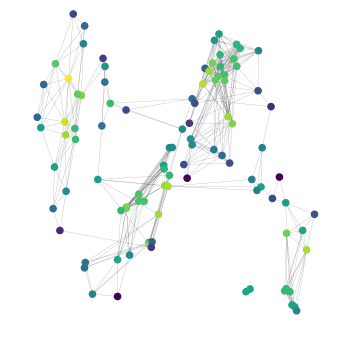
\includegraphics[width=0.22\linewidth]{img/cgcn_conv_illus0crop.png}
%  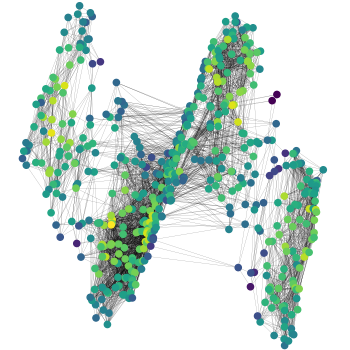
\includegraphics[width=0.22\linewidth]{img/cgcn_conv_illus1crop.png}
%  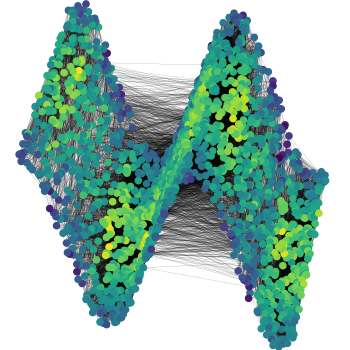
\includegraphics[width=0.22\linewidth]{img/cgcn_conv_illus2crop.png}
%  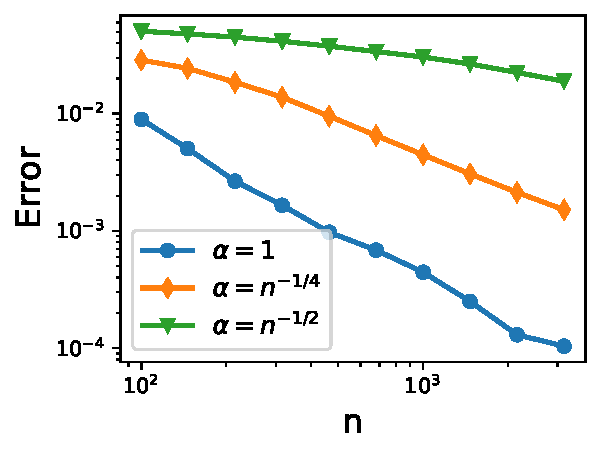
\includegraphics[width=0.25\linewidth]{img/cgcn_convergence.pdf}
%\end{myalertblock}

\end{column}



















%%%%%%%%%%%%%%%%%%%%%%%%%%%%%%%%%%%%%%%%%%%%

\begin{column}{0.29\linewidth}
\begin{myalertblock}{4: Stability of GCNs to model deformations}

For $i = 1,2$, assume $(A_{i},Z_{i})$ drawn from models $(W_{i}, P_{i}, f_{i})$.

\hspace*{.01\linewidth}\begin{minipage}{.96\linewidth}
\begin{mynotablock}{Finite-sample stability in the equivariant case}

\mycolback{
  \textbf{Theorem}
  Denote $Q_i = \Phi_{W_i,P_i}(f_i)_\sharp P_i$. With prob. $1-n^{-r}$:
  \begin{align*}
  &\mathsmaller{\min_{\sigma \in \Sigma_n} \sqrt{\frac{1}{n} \sum_i ((\Phi_{A_1})_i - (\Phi_{A_2})_{\sigma(i)})^2}} \\
    &\qquad  \qquad \qquad \leq \mathcal{W}_2(Q_1,Q_2) + R_n + O(n^{-1/d}),
  \end{align*}
  where~$\mathcal{W}_2$ is the Wasserstein-2 distance and~$d = \text{dim}(\Xx)$.
}

\end{mynotablock}
\end{minipage}

\vspace{0.5cm}

\hspace*{.01\linewidth}\begin{minipage}{.96\linewidth}
\begin{mynotablock}{Deformation of a translation-invariant model}
\begin{itemize}
  \item Translation-invariant kernel $W(x,y) = w(x-y)$
  \item Smooth diffeomorphism [3] $\tau: \mathcal{X} \to \mathcal{X}$ (``size'' $\|\nabla \tau\|_\infty$)
\end{itemize}
% Translation-invariant kernel $W(x,y) = w(x-y)$, deformation $\tau: \mathcal{X} \to \mathcal{X}$.

\vspace{0.5cm}
\mycolback{
  \textbf{Theorem} (Deformations of~$W$, $P$, or~$f$.)
  \begin{itemize}
  \item $W(x, x') \to W_\tau(x, x') \eqdef W(x - \tau(x), x' - \tau(x'))$
  \[\|\bar \Phi_{W_\tau} - \bar \Phi_{W}\| \lesssim \|\nabla \tau\|_\infty\]
  \item $P \to P_\tau = (Id-\tau)_\sharp P$, and $f' = f \circ (Id- \tau)$, or degree functions as inputs $(f, f') = (d_P, d_{P_\tau})$
  \[\|\bar \Phi_{P}(f) - \bar \Phi_{P_\tau}(f')\| \lesssim \|\nabla \tau\|_\infty\]
  \item $f \to f_\tau = f \circ (Id-\tau)$
  \[\|\bar \Phi(f_\tau) - \bar \Phi(f)\| \lesssim \|\nabla \tau\|_\infty.\]
  \end{itemize}
  Similar bounds hold for the equivariant case on~$\mathcal W_2(Q_1, Q_2)$ with $Q_i = \Phi_{W_i,P_i}(f_i)_\sharp P_i$.
}
\end{mynotablock}
\end{minipage}

\vspace{2cm}
Numerical illustration (Random graph with 3D latent positions)\\
  \small
  From left to right: output signal; new drawing of the random edges; deterministically deformed latent positions; invariant GCN with respect to the amplitude of the deformation.\\
  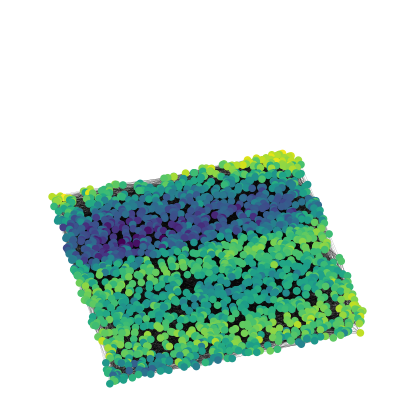
\includegraphics[width=0.22\linewidth]{img/stab_figcrop.png}
  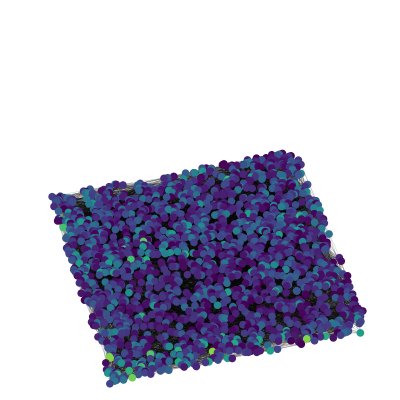
\includegraphics[width=0.22\linewidth]{img/stab_fig1crop.png}
  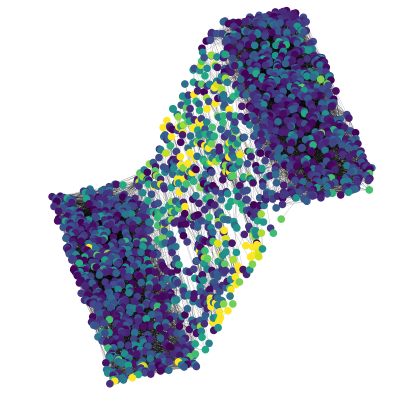
\includegraphics[width=0.22\linewidth]{img/stab_fig0crop.png}
  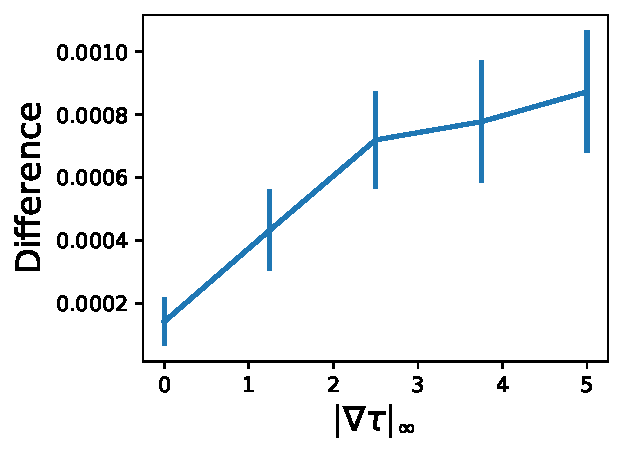
\includegraphics[width=0.28\linewidth]{img/illus_stab.pdf}
\end{myalertblock}

% \begin{block}{Numerics (synthetic)}
% Random graphs with 3D latent positions.\\
% \textbf{Convergence of GCN}\\
%   \small
%   Input signal $f=1$ with growing number of nodes (left) and convergence with different sparsity levels $\alpha_{n}$ (right)\\
%   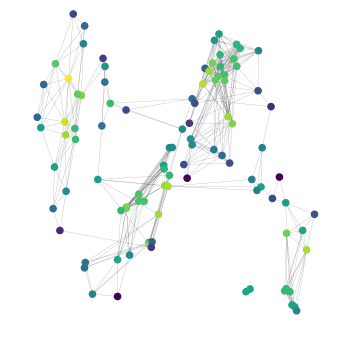
\includegraphics[width=0.22\linewidth]{img/cgcn_conv_illus0crop.png}
%   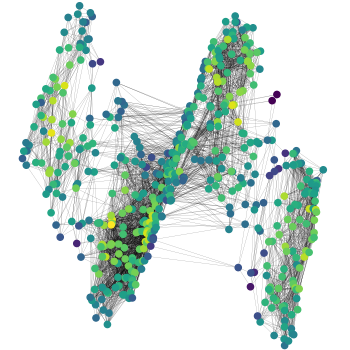
\includegraphics[width=0.22\linewidth]{img/cgcn_conv_illus1crop.png}
%   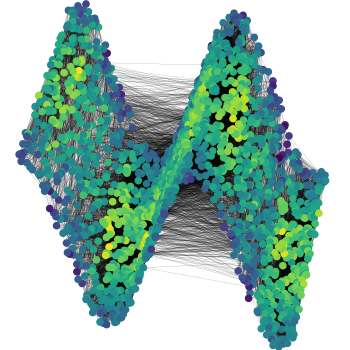
\includegraphics[width=0.22\linewidth]{img/cgcn_conv_illus2crop.png}
%   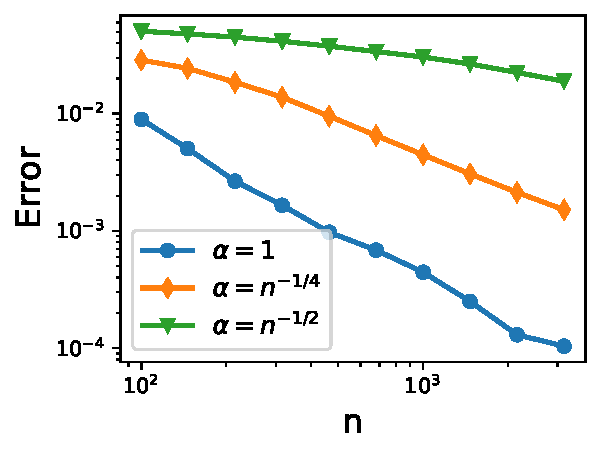
\includegraphics[width=0.25\linewidth]{img/cgcn_convergence.pdf}

% \textbf{Stability of GCN}\\
%   \small
%   From left to right: output signal; new drawing of the random edges; deterministically deformed latent positions; invariant GCN with respect to the amplitude of the deformation.\\
%   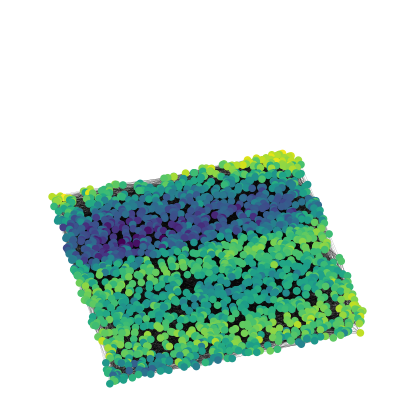
\includegraphics[width=0.22\linewidth]{img/stab_figcrop.png}
%   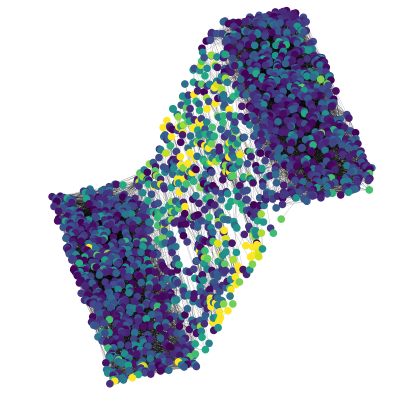
\includegraphics[width=0.22\linewidth]{img/stab_fig0crop.png}
%   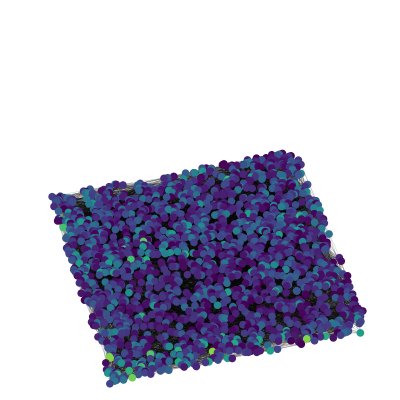
\includegraphics[width=0.22\linewidth]{img/stab_fig1crop.png}
%   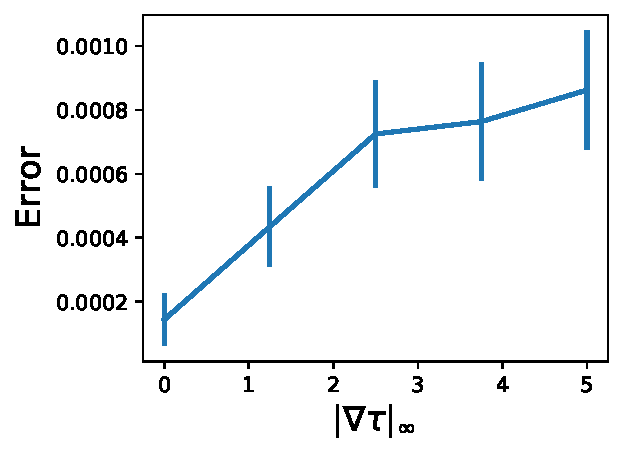
\includegraphics[width=0.25\linewidth]{img/cgcn_stability.pdf}
% \end{block}


% \begin{block}{References}

 {\footnotesize
   \begin{itemize}
   \item[{[1]}]Bruna et al. \textbf{Spectral Networks and Locally Connected Networks on Graphs}. \emph{ICLR}, 2014.
   \item[{[2]}] Xu et al. \textbf{How Powerful are Graph Neural Networks?}. \emph{ICLR}, 2020.
   \item[{[3]}] Mallat. \textbf{Group Invariant Scattering}. \emph{Comm. Pure Appl. Math.}, 2012.
	\item[{[4]}] Gama et al. \textbf{Stability Properties of Graph Neural Networks}. \emph{IEEE Trans. Sig. Proc.}, 2020.
	
\end{itemize}
 }

% \end{block}%2


\end{column}
\end{columns}




\end{frame}
\end{document}
